\begin{frame}
\frametitle{\mTtot\ distributions}

\begin{minipage}[t]{.49\textwidth}

\manip Backgrounds = SM expectations:
\submanip DY $\Zboson\to\tau\tau$ and some \ttbar\ in \colorbox{\EMBcolor}{$\mu\to\tau$ embedded}
\submanip QCD, \Wjets\ and some \ttbar\ in \colorbox{\FAKEScolor}{$\text{Jet}\to\tauh$}
\submanip $\Zboson\to\ele\ele$ + $\Zboson\to\mu\mu$ in \colorbox{\ZLLcolor}{$\Zboson\to\ell\ell$}
\submanip Remaining \ttbar\ in \colorbox{\TTBARcolor}{\ttbar}
\submanip Other small backgrounds in \colorbox{\DIBcolor}{Diboson}

\only<2->{\manip \Higgs\ at \SI{400}{\GeV} expected $\sigma\times\BR=\SI{1}{\pico\barn}$ \tikzmarknode{signal.}{nodesignal}}

\only<3->{\manip Compare to observed events (black dots).}

%\vspace{\baselineskip}
%
%\manip Lots of work to obtain this!
%\submanip simulated events
%\submanip detector issues
%\submanip uncertainties measured
%\manip Collaboration with KIT (Germany)
%
%\vspace{\baselineskip}

\only<5->{\manip Data/Bkg agreement $\to$ \textbf{exclusion limits} on $\sigma\times\BR$}
\end{minipage}
\hfill
\begin{minipage}[t]{.49\textwidth}
\begin{center}
\vspace{-2\baselineskip}

%\only<1>{\plotHTTshapes{mt_tot}{mssm_classic}{2018}{tt}{32}{prefit_nosignal_blinded}}
\only<1-2>{\plotHTTshapes{mt_tot}{mssm_classic}{2018}{tt}{32}{prefit_blinded}}
\only<3->{\plotHTTshapes{mt_tot}{mssm_classic}{2018}{tt}{32}{prefit}}
\end{center}
\end{minipage}

\begin{tikzpicture}[overlay, remember picture]
\only<2>{
\draw [ltcolorred, very thick, -latex] (nodesignal) to [out=0, in=-165] (11.45,5);
}
\only<4>{
\fill [white, opacity=.9] (0,0) rectangle (.5\textwidth, .85\textheight);
\draw (.025\textwidth, .7\textheight) node [right, text depth=0pt] (A) {\manip \textbf{Lot} of hard work to obtain this:};
\draw (A.north) node [above] {\textbf{Not \emph{just} a plot!}};

\foreach \txt in {simulated events, detector issues, uncertainties measured}{
\draw (A.south west) node [below right] (A) {\submanip \txt};
}
\draw (A.south west) node [below right] (A) {\manip Collaborative work:};
\foreach \txt in {Karlsruhe Institute of Technology (DE), Imperial College (UK), DESY (DE), HEPHY (AT), IP2I (FR)}{
\draw (A.south west) node [below right] (A) {\submanip \txt};
}
}
\end{tikzpicture}
\end{frame}

\begin{frame}
%\frametitle{Exclusion limits}
\beamercite{CLs_method}

\begin{minipage}[c]{.49\textwidth}
\begin{center}
\only<1-6>{\plotHTTModelIndepLimits{mssm_classic}{combined}{ggH}{_cmb}}
\only<7->{\plotHTTModelIndepLimits{mssm_classic}{combined}{ggH}{_cmb_vs_CMS_ATLAS}}
\end{center}
\end{minipage}
\hfill
\begin{minipage}[c]{.49\textwidth}
\begin{center}
\only<2-5>{\plotHTTshapes{mt_tot}{mssm_classic}{2018}{tt}{32}{prefit}}
\only<6>{\plotHTTModelIndepLimits{mssm_classic}{combined}{bbH}{_cmb}}
\only<7->{\plotHTTModelIndepLimits{mssm_classic}{combined}{bbH}{_cmb_vs_CMS_ATLAS}}
\end{center}
\end{minipage}

\begin{tikzpicture}[overlay, remember picture]
\only<2-4>{
\draw [ltcolorred, very thick] (.935\textwidth, .5\textheight) circle (.4) ;
\draw [ltcolorred, thick, dotted] (3.56,1) --+ (0, 3.9);
}

\only<3-4>{
\draw [ltcolorred, very thick, latex-] (11.45, 4.8) --+ (0, -.4);
\draw [ltcolorred, very thick, latex-] (11.45, 5.1) --+ (0, .4) node [above] {\small $\sigma\times\BR=\SI{1}{\pico\barn}$};
}

\only<4>{
\def\ypos{4.28}
\draw [ltcolorred, thick, dotted] (1.3, \ypos) --+ (6,0);
\draw [ltcolorred, very thick] (11.45,4.95) ellipse (.3 and .6) ;
\fill [ltcolororange] (3.56,\ypos) circle (3pt) ;
\draw [ltcolorred, very thick, -latex] (11.15,4.95) to [out=-180, in = 0] (3.56,\ypos) ;
}

\only<5>{
\draw [ltcolorred] (3.56,4) node [right] {Would have been seen} ;
\draw [ltcolorred] (3.56,2) node [left] {Can't tell} ;
}
\end{tikzpicture}
\end{frame}

\begin{frame}
%\frametitle{Model-dependant limits}

\begin{minipage}[c]{.49\textwidth}
\only<1>{\manip Model dependent limits:
\submanip Fix high-order MSSM parameter,
\submanip Explore $(m_{\HiggsA},\tan\beta)$ plane,
\submanip Do data stick more to SM or MSSM?}
\only<2>{
\begin{center}
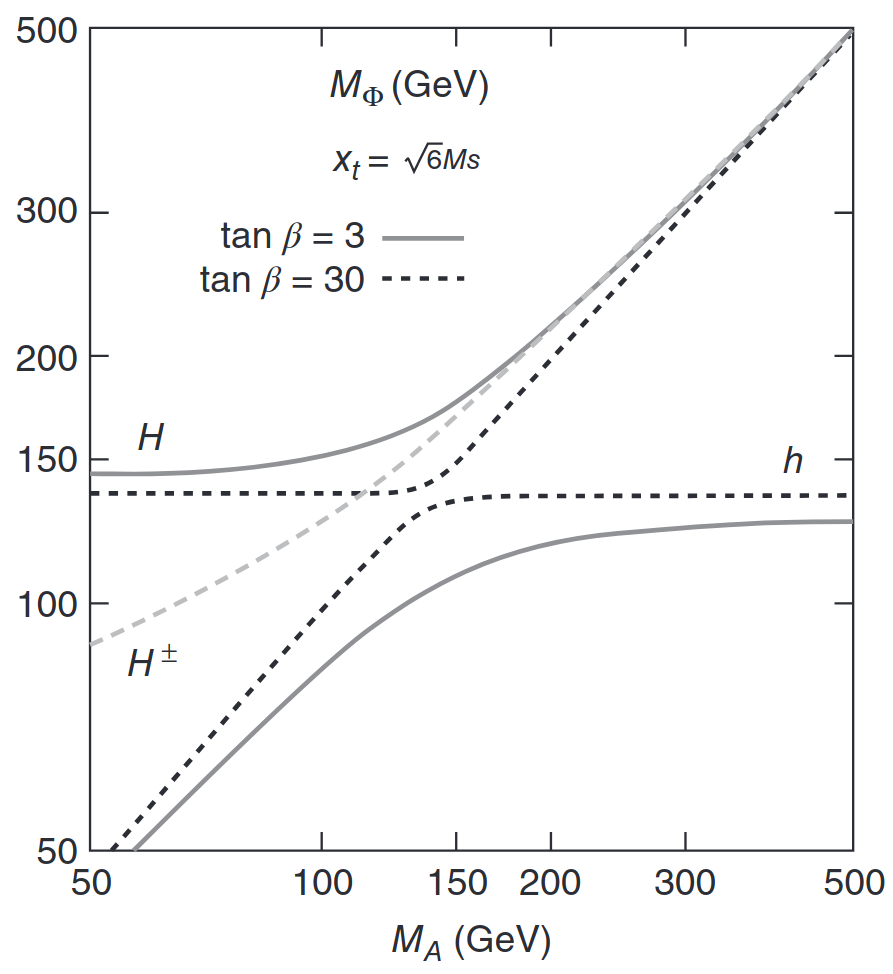
\includegraphics[height=\graphh]{\PhDthesisdir/plots_and_images/from_Nagashima_BSM/fig_1-9.tex}
\end{center}
}
\end{minipage}
\hfill
\begin{minipage}[c]{.49\textwidth}
\begin{center}
\plotHTTModelDepLimits{mssm_vs_sm_h125}{_vs_CMS}
\end{center}
\end{minipage}

\begin{tikzpicture}[overlay, remember picture]
\draw [ltcolorred] (10.5,4) node {data = more SM-like} ;
\draw [ltcolorred] (14,2.5) node {Can't tell} ;
\end{tikzpicture}

\end{frame}